\chapter{Design}\label{C:des}

This project's scope is concerned with the development and experimentation of the two core components that make up this system. These are The Feature Extractor and The Predictor. Although this project is relatively immature, I have paid some respects to the theoretical end-solution at each project stage. This was important as it relates to the motivation behind the project - to provide the stakeholders with a usable tool. In saying this, the following diagram is a naive representation of the theoretical end-solution or product. 

\begin{figure}[h]
     \centering
     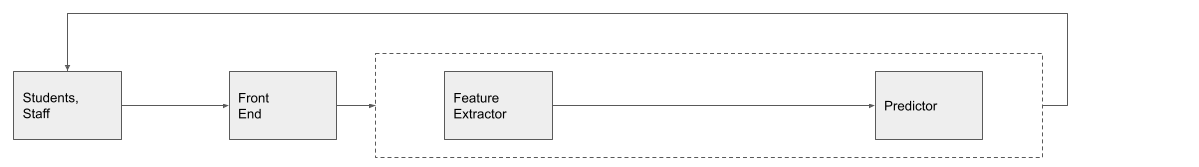
\includegraphics[width=.8\linewidth]{pngs/prod.png}
     \caption{AES as a Product}\label{Fig:Data1}
\end{figure}

As for the scope of this project, as mentioned previously, it is concerned with the development and experimentation of the Feature Extractor and The Predictor. Additionally, as with any machine learning endeavor, it heavily relies on relevant data to develop, test, and evaluate. Therefore, another critical in this investigation is The Prediction Configuration Generator (PCG). The PCG, paired with The Predictor and The Error Calculator, allowed for extensive exploration, insight, and evaluation of the system. 

\begin{figure}[h]
     \centering
     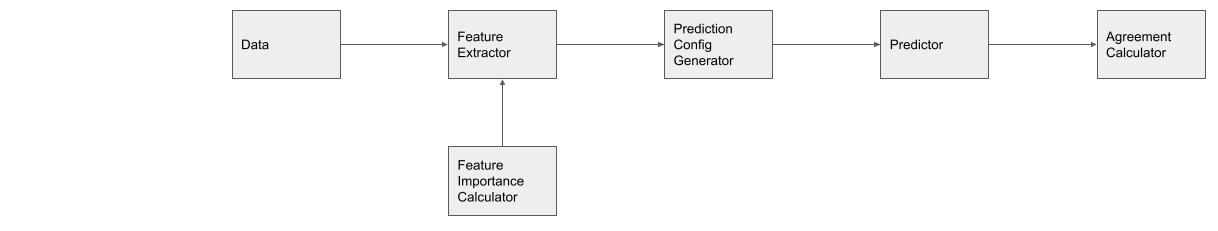
\includegraphics[width=.8\linewidth]{pngs/dev.png}
     \caption{AES in Development}\label{Fig:Data1}
\end{figure}

\section{The Data}
Preparing the data for the Feature Extractor can be broken down into three main stages - discovery, digitising, and processing. The product of these stages is the structured digital representation of an essay given to the Feature Extractor.

\begin{figure}[h]
     \centering
     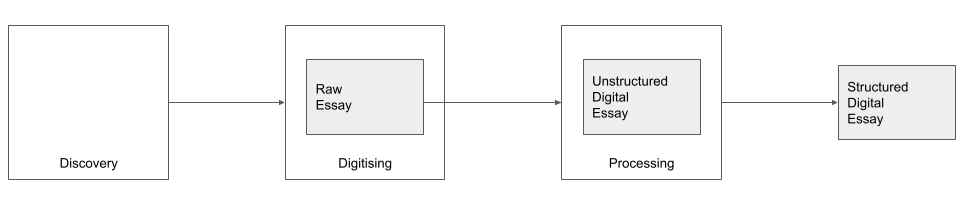
\includegraphics[width=.75\linewidth]{pngs/data-stages.png}
     \caption{The Data: Stages}\label{Fig:Data1}
\end{figure}

\subsection{Discovery}
The discovery step was mainly concerned with discovering relevant data sets to be used for the project. The Hewlett foundation competition data was used in the early stages of the project. As it progressed, the Victoria University of Wellington: English Proficiency Program data was acquired.

% Please add the following required packages to your document preamble:
% \usepackage{booktabs}
\begin{table}[h]
\centering
\begin{tabular}{@{}|l|llllllll|l|@{}}
\toprule
Dataset &
  \multicolumn{8}{l|}{Hewlett} &
  VUW \\ \midrule
Total Essays &
  \multicolumn{1}{l|}{1,785} &
  \multicolumn{1}{l|}{1,800} &
  \multicolumn{1}{l|}{1,726} &
  \multicolumn{1}{l|}{1,772} &
  \multicolumn{1}{l|}{1,805} &
  \multicolumn{1}{l|}{1,800} &
  \multicolumn{1}{l|}{1,730} &
  918 &
  113 \\ \midrule
Average Words &
  \multicolumn{1}{l|}{350} &
  \multicolumn{1}{l|}{350} &
  \multicolumn{1}{l|}{150} &
  \multicolumn{1}{l|}{150} &
  \multicolumn{1}{l|}{150} &
  \multicolumn{1}{l|}{150} &
  \multicolumn{1}{l|}{250} &
  650 &
  376 \\ \bottomrule
\end{tabular}
\caption{Dataset Statistical Overview}
\label{tab:1}
\end{table}

\paragraph{The Victoria University of Wellington: English Proficiency Program}
The Victoria University of Wellington: English Proficiency Program (VUW EPP) dataset consists of 113 essays with scores for each of the following categories, which were triple marked: grammar, vocab, flow, ideas, coherence, overall. This dataset initially consisted of two separate sets and was joined into one. Each set is from a trimester of the written assessment component of the EPP program.

\paragraph{The Hewlett Foundation}
The Hewlett Foundation dataset Competition consists of eight essay sets. Each of the essay collections was born from a particular prompt. The length of selected essays varies from 150 to 550 words per response. Some of the writings rely on information from sources, while others do not. All of the replies were submitted by kids in grades 7 through 10, and they ranged in age from 7 to 10. All essays were double-scored and assessed by hand. Thus, each of the eight data sets is distinct in its way. 
 
\subsection{Digitisation}
The digitisation stage mainly consisted of converting handwritten essays to digital word documents. The essay format from the data from the Victoria University of Wellington: English Proficiency Program was handwritten. This was done by manually transcribing each essay using text-to-speech to multiple word documents. The scores from this dataset were in the format of a printed document. This was digitized manually through data entry to a spreadsheet document.

\subsection{Processing}
The processing stage consisted of converting unstructured-digital data into structured data. Throughout this task, I tried to automate as much as possible to save time and reduce the risk of human error. The implementation required for this stage is discussed further in the implementation section.

The data in this project consists of two common format types - Comma-Separated Values (CSV) and Tab-Separated Values (TSV). The main difference between them is simply the identifier that the information is separated with - either a comma or a tab. They are both widely used for many purposes and are primarily encountered in spreadsheets and databases. I chose to use them because they are widely used and, as a result, can be easily interpreted by many different programs or tools, such as spreadsheet processors. These were used to manipulate the data manually—also, Python, where libraries already existed to easily interpret and parse data with this structure.

The target structure is to have one essay per row, with its respective information following on the same row, in the following order: the id, the text of the essay, and then the scores associated with that essay. Of course, the scores will vary depending on the dataset. 

% Please add the following required packages to your document preamble:
% \usepackage{booktabs}
\begin{table}[h]
\centering
\begin{tabular}{@{}|l|l|lllll|@{}}
\toprule
id & essay & \multicolumn{5}{l|}{scores}                                                                      \\ \midrule
   &       & \multicolumn{1}{l|}{} & \multicolumn{1}{l|}{} & \multicolumn{1}{l|}{} & \multicolumn{1}{l|}{} &  \\ \bottomrule
\end{tabular}
\caption{Structured Data Table Format}
\label{tab:2}
\end{table}

\section{The Feature Extractor}

The Feature Extractor is responsible for identifying, calculating, categorizing, and numerically representing the "features" of a given essay so that they can be inputted into other components to produce computer-generated scores. For example, the following figure depicts how The Feature Extractor takes a structured essay as input and produces multiple feature categories.  

% \begin{center}
%     \includegraphics[scale=.15]{design-the-feature-extractor.png}
% \end{center}

A feature category is simply a TSV file containing a row for every essay from the inputted structured essay data and columns for the respective ids, scores, and features relevant to the category. For example, for most executions, the feature extractor will output six TSV files for each category. Each file will contain a row for every essay, although the columns will vary as they will only contain the features for their respective category. The figure below is a visual representation of this table structure. 

% Please add the following required packages to your document preamble:
% \usepackage{booktabs}
\begin{table}[h]
\centering
\begin{tabular}{@{}|l|lllllll|lllll|@{}}
\toprule
id &
  \multicolumn{7}{l|}{features} &
  \multicolumn{5}{l|}{scores} \\ \midrule
 &
  \multicolumn{1}{l|}{} &
  \multicolumn{1}{l|}{} &
  \multicolumn{1}{l|}{} &
  \multicolumn{1}{l|}{} &
  \multicolumn{1}{l|}{} &
  \multicolumn{1}{l|}{} &
   &
  \multicolumn{1}{l|}{} &
  \multicolumn{1}{l|}{} &
  \multicolumn{1}{l|}{} &
  \multicolumn{1}{l|}{} &
   \\ \bottomrule
\end{tabular}
\caption{Feature Category Table Format}
\label{tab:3}
\end{table}

\subsection{Categories}
The categories are based on the EEP marking criteria to optimize the prediction of these same categories by organizing each feature into a group or category based on their relevance with these same categories. For example, categorizing the count of grammatical errors of an essay into the grammar feature category will very likely aid in depicting an essay's proficiency within this category and, therefore, the system's ability to predict such a mark. 

\subsection{Resources}
The Feature Extractor uses three predefined resources to help calculate several specific functions. These resources are described below.

\paragraph{Headwords and Basewords} The Headwords and Basewords resource consist of 25,000 headwords and basewords from The Corpus of Contemporary American English (COCA) and the British National Corpus (BNC). Headwords are essential to the core meaning of a phrase, for example, "create." Basewords can be thought of as variations of this word, for example, "create," "creation," "creative." The COCA and the BNC complement each other nicely, and they are only large, well-balanced corpora of English that are publicly available. The BNC has better coverage of informal, everyday conversation, while COCA is much larger and more recent, which has important implications for the quantity and quality of the data overall. The lists are designed primarily for learners of English as a foreign language [16]. 

\paragraph{Stopwords} The Stopwords resource consists of a list of stopwords from the Natural Language Toolkit Python library. Stopwords are a set of commonly used words in a language. Examples of stop words in English are "a", "the", "is", "are", and "etc".

\paragraph{POS Trigrams} The POS Trigrams resource consists of a list of Trigrams. A trigram is a contiguous sequence of three items from a given sample of text or speech. These items can be phonemes, syllables, letters, words, or base pairs according to [based] on the application. The items in this list only consist of part-of-speech identifiers, such as; nouns, verbs, adjectives, adverbs. This list was imported from the Travis Moore study. He found that from a particular set of POS trigrams, there was a correlation between the amount of these trigrams an essay contained and its score [17]. 

\subsection{The Features}
For every essay, the following features are calculated and categorized. Below is a summary of every feature and its respective category. More information about the implementation of the extraction or calculation of these can be found in the feature extraction section of the implementation section. Most features from this section are derived from the Travis Moore study [17].

\subsubsection{Miscellaneous}
This category contains some elementary features that I chose not to categorize, but instead, they are added to every category. This category is not part of the exported feature categories. The produced features include:
\begin{itemize}
 \item The total words
 \item The total sentences
 \item The total words per sentence
 \item The sentences per 100 words
\end{itemize}

\subsubsection{Grammar }

\paragraph{Transition Words}
Transition words are words that help connect or link ideas, phrases, sentences, or paragraphs. These words help the reader smoothly through ideas by creating a bridge between them. The transition words of the essay  are used to produce the following features:
\begin{itemize}
 \item The percentage of the transition words in the essay out of the Transitions Set. 
\end{itemize}

\paragraph{Parts of Speech Trigrams}The POS Trigrams Resource is used to find matches in the essay, and then the count of matches is the percentage of Parts of Speech trigrams found in the essay from the "relevant trigrams set."

\subsubsection{Vocab }

\paragraph{Difficult Words} The difficult words are discovered using the Python Textstat library (explained further below) and are used to produce the following features:
\begin{itemize}
 \item The total difficult words in the essay
\end{itemize}

\paragraph{Headwords and Basewords} The Headwords and Basewords resource is separated into multiple lists. Then, for each list, the words from the list and the essay are compared to produce the following features:
\begin{itemize}
 \item The words in both divided by the list length
 \item The words in both divided by the total words of the essay
\end{itemize}

\paragraph{Unique Words}
Unique words are defined as being the only one of their kind and are used to produce the following features:
\begin{itemize}
 \item The total unique words in the essay
 \item The average unique words (total unique divided by the total words)
 \item The number of unique words per 100 words
\end{itemize}

\subsubsection{Flow}
\paragraph{Readability Counts} Textstat is used to produce the following counts:
\begin{itemize}
 \item Total sentences
 \item Total characters
 \item Total letters 
\end{itemize}

\paragraph{Syllables} The syllables in each word of the essay are used to process the following features:
\begin{itemize}
 \item The total syllables
 \item The number of words with a syllable count greater than two
 \item The number of words with a syllable count equal to one
\end{itemize}

\paragraph{Reading Time}The time it would take to read the essay

\paragraph{Readability Consensus}The estimated school grade level required to understand the text 

\paragraph{Readability Scores}
Using Textstat's readability measures, the following features are produced:
\begin{itemize}
 \item The Flesch Reading Ease
 \item The Flesch-Kincaid Grade Level
 \item The Fog Scale Returns the FOG
 \item Spache Readability Formula
 \item The SMOG Index
 \item The Coleman-Liau Index
 \item Automated Readability Index 
 \item Linear Write Formula
 \item Dale-Chall Readability Score
\end{itemize}

\subsubsection{Coherence}
\paragraph{Lemmas}
A lemma is a canonical form, dictionary form, or citation form of a set of words. The lemmas of the essay are used to produce the following features:
\begin{itemize}
 \item Total Lemmas 
 \item Total Lemmas from Unique Words 
 \item Total Brigrams from Lemmas
 \item Total Brigrams from Lemmas from Unique Words 
 \item Total Trigrams from Lemmas
 \item Total Trigrams from Lemmas from Unique Words 
\end{itemize}

\paragraph{Content Words}
Content words, in linguistics, are words that possess semantic content and contribute to the meaning of the sentence in which they occur. The content words are discovered by removing all stopwords from the text. The content words of the essay are used to produce the following features:
\begin{itemize}
 \item The total content words
 \item The total unique content words
 \item The percentage of unique content words out of the non-unique content words found 
\end{itemize}

\paragraph{Function Words}
Function words are words that have little lexical meaning or have ambiguous meaning and express grammatical relationships among other words within a sentence or specify the attitude or mood of the speaker. They signal the structural relationships that words have to one another and are the glue that holds sentences together. Thus they form essential elements in the structures of sentences. The function words of the essay are used to produce the following features:
\begin{itemize}
 \item The total function words
 \item The total unique function words
\item The percentage of unique function words out of the non-unique functions found \end{itemize}

\paragraph{Nouns}
\begin{itemize}
 \item The nouns of the essay are used to produce the following features:
 \item The total nouns 
 \item The total unique nouns
 \item The percentage of unique nouns out of the non-unique nouns found
\end{itemize}

\paragraph{Determiners}
A determiner is a modifying word that determines the kind of reference a noun or noun group has, for example, "a," "the," "every." The determiners of the essay are used to produce the following features:
\begin{itemize}
 \item The total determiner
 \item The total unique determiner
 \item The percentage of unique determiner out of the non-unique determiners found
\end{itemize}

\paragraph{Conjunctions}
A conjunction is a word used to connect clauses or sentences or coordinate words in the same clause. For example, "but", "if". The conjunctions of the essay are used to produce the following features:
\begin{itemize}
 \item The total conjunctions 
 \item The total unique conjunctions
 \item The percentage of unique conjunctions out of the non-unique conjunctions found
\end{itemize}

\paragraph{Pronouns}
A pronoun is a word that can function as a noun phrase used by itself, and that refers to the participants in the discourse, for example, "I," "you," or to someone or something mentioned elsewhere in the discourse, for example, "she," "it," "this." The pronouns of the essay are used to produce the following features:
\begin{itemize}
 \item The total pronouns 
 \item The total unique pronouns
 \item The percentage of unique pronouns out of the non-unique pronouns found
\end{itemize}

\subsubsection{Ideas }
This category does not contain any unique features. 

\subsubsection{Overall}
This category contains the features from all of the previous categories.

% \begin{wrapfigure}{r}{0.4\textwidth}
%   \begin{center}
%     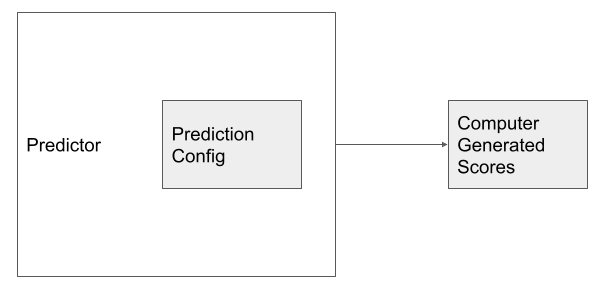
\includegraphics[width=0.3\textwidth]{pngs/predictor-1111.png}
%   \end{center}
%   \caption{The Predictor}\label{Fig:Data1}
%   \end{wrapfigure}

\section{The Predictor}

The Predictor is responsible for producing computer-generated scores. As described in the following figure, it takes a prediction configuration as input and produces scores based on this configuration.

\begin{figure}[h]
  \begin{minipage}{0.48\textwidth}
     \centering
     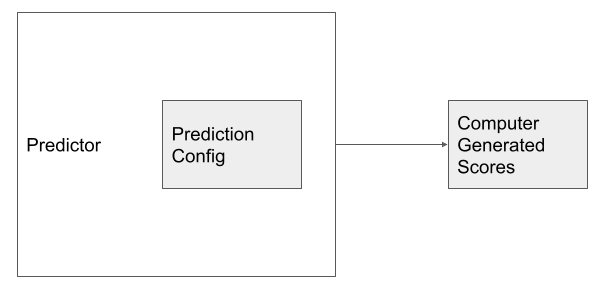
\includegraphics[width=.7\linewidth]{pngs/predictor-1111.png}
     \caption{The Predictor}\label{Fig:Data1}
  \end{minipage}\hfill
  \begin{minipage}{0.48\textwidth}
     \centering
     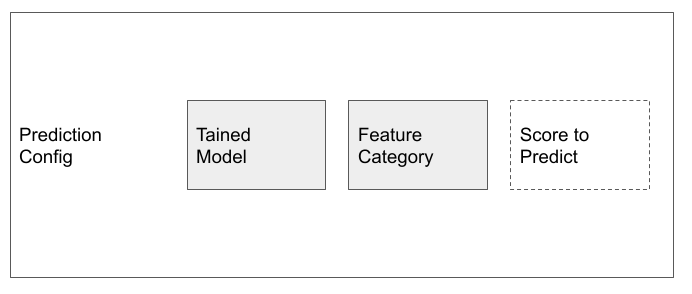
\includegraphics[width=.7\linewidth]{pngs/prediction-config.png}
     \caption{Prediction Configuration}\label{Fig:Data2}
  \end{minipage}
\end{figure}

% \begin{wrapfigure}{r}{0.4\textwidth}
%   \begin{center}
%     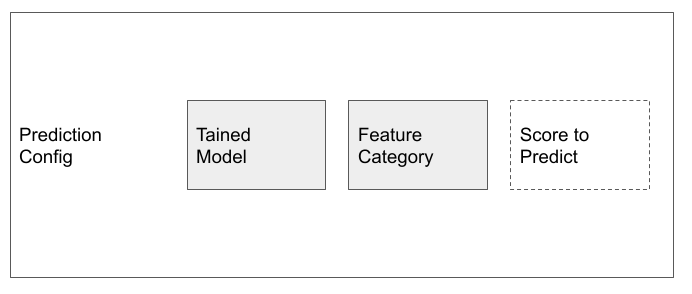
\includegraphics[width=0.3\textwidth]{pngs/prediction-config.png}
%   \end{center}
%   \caption{The Predictor}\label{Fig:Data1}
%   \end{wrapfigure}

\subsection{Prediction Configuration}

A Prediction Configuration, as seen below, is composed of a trained model, a feature category, and the target score to predict from the feature category. A trained model is a model which has an enhanced understanding of a relationship between an input and an output for a specific problem by being given examples of this problem from a specific dataset.  

% \begin{figure}[h]
%      \centering
%      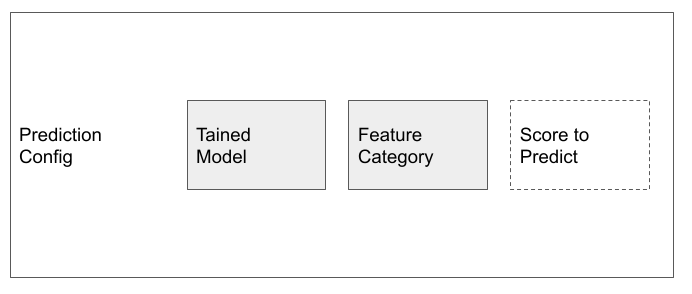
\includegraphics[width=.4\linewidth]{pngs/prediction-config.png}
%      \caption{AES as a Product}\label{Fig:Data1}
% \end{figure}

\subsection{The Prediction Configuration Generator}
The Prediction Configuration Generator (PCG)  is responsible for producing multiple prediction configuration objects. It can also be used to produce a single prediction configuration object, which may be useful after the evaluation stage of this project. 

For the experimental stage of this project, it was advantageous to produce prediction configuration permutations because it allowed us to explore the a variety of  Prediction Configurations. 

\begin{figure}[h]
   \begin{minipage}{0.48\textwidth}
     \centering
     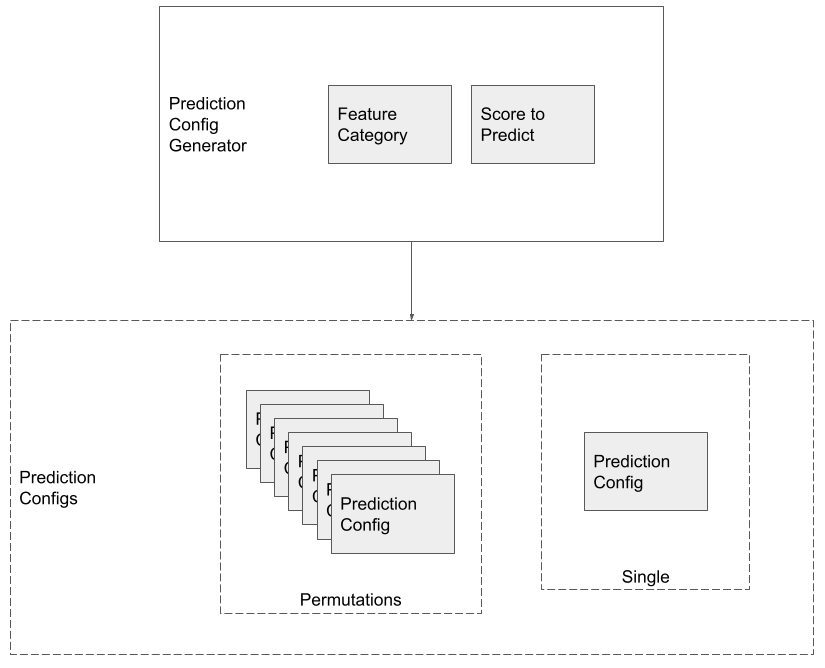
\includegraphics[width=.7\linewidth]{pngs/pcg-permutations.png}
     \caption{PCG: Permutator}\label{Fig:Data1}
   \end{minipage}\hfill
   \begin{minipage}{0.48\textwidth}
     \centering
     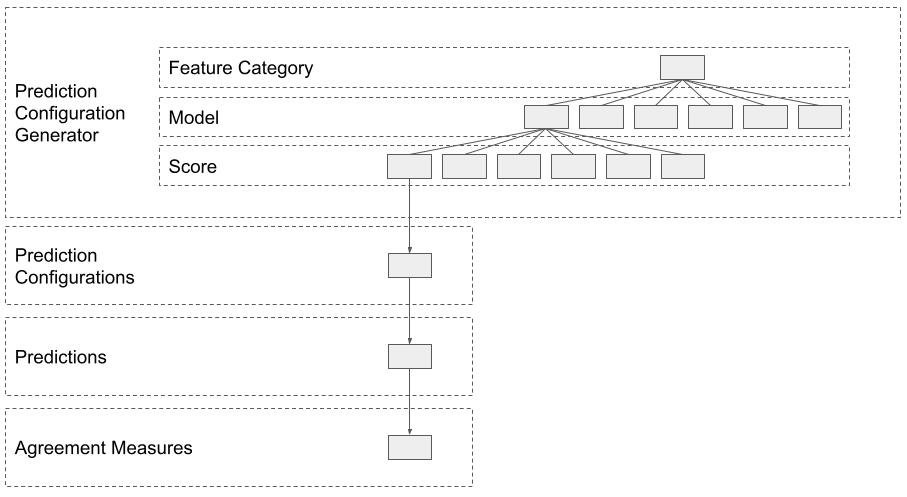
\includegraphics[width=.7\linewidth]{pngs/pcg-tree.png}
     \caption{PCG: Pipeline}\label{Fig:Data2}
   \end{minipage}
\end{figure}